\documentclass[main.tex]{subfiles}

\begin{document}

  \section{Computational aspects}

   \subsection{Complexity analysis}

   We recall the parameters of the problem: we consider a superelliptic curve
   $\cu=y^m=f(x)$ where $f$ has degree $d$. It has genus $g$, where
   $g\leq \frac{(m-1)(d-1)}2=O(md)$.

   Let $D$ be some desired accuracy (a number of digits). The computation of
   the Abel-Jacobi map on $\cu$ has been decomposed into the
   following list of tasks:
   \begin{enumerate}
       \item computing the $(d-1)$ elementary integrals
       \item computing the big period matrix $\Omega=(\OA,\OB)$ \eqref{eq:OAOB}
       \item computing the small period matrix $\tau$ \eqref{eq:tau}
       \item evaluating the Abel-Jacobi map at a point $P$
   \end{enumerate}
   all of these to absolute precision $D$.

   Let $n(D)$ be the number of points of numerical integration.
   If $m=2$, we have
   $n(D)=O(D)$ using Gauss-Chebychev integration, while $n(D)=O(D\log D)$
   via double exponential integration.

   For multiprecision numbers, we consider that the multiplication has
   complexity $M(D)=O(D\log D)$,
   while simple transcendental functions (log, exp, sinh,\dots) can be evaluated
   in complexity $T(D)=O(D\log^2 D$).

   \subsubsection{Computation of elementary integrals}

   For each elementary cycle $\gamma_e\in C$, we evaluate numerically the $g$
   integrals of differentials from \eqref{m-eq:thm_periods} as sums of the form
   \begin{equation}
       \int_{-1}^1\frac{\varphi_{i,j}(u)\du}{(1-u^2)^{\frac jm}}
           \approx \sum_{k=1}^n w_k\frac{x_k^{i-1}}{y_k^j}
   \end{equation}
   where $n$ is the number of integration points, $w_k,u_k$ are integration weights and points,
   $x_k=u_k+\frac{b+a}{b-a}$ and $y_k=\ytab(u_k)$.

   We proceed as follows:
   \begin{itemize}
       \item we compute the integrals of all $g$ differentials at the same time;
   \item for each point $k$, we evaluate the absissa and weights $u_k,w_k$ using
       a few trigonometric or hyperbolic functions\footnote{this can be reduced to only one exponential
       and a few multiplications};
   \item we compute $y_k=\ytab(u_k)$ using $d-3$ multiplications and one $m$th root,
       as shown in section \ref{sec:computingroots} below;
   \item starting from $\frac{w_k}{y_k}$, we evaluate all $g$ terms $w_k\frac{x_k^{i-1}}{y_k^j}$
       each time either multiplying by $x_k$ or dividing by $y_k$, and add each to the corresponding
       integral.
   \end{itemize}

   All in all, the computation of one elementary integral takes $nT(D)+n(d-3)M(D)+ngM(D)$ operations,
   so that depending on the integration scheme we obtain
   \begin{thm}
       \label{thm:complexity_integrals}
       Each of the $(d-1)$ elementary integrals can be computed to precision $D$ using
       \begin{itemize}
           \item $O(D^2\log D (g + \log D))$ operations if $m=2$
           \item $O(D^2\log D (g + \log^2 D))$ operations if $m>2$
       \end{itemize}
   \end{thm}

   \subsubsection{Big period matrix}

   One of the nice aspects of the method is that we never compute
   the dense matrix $\OC\in\C^{g\times 2g}$ from \eqref{eq:OC}, but
   keep the decomposition of periods in terms of the elementary integrals
   $\int_{\gamma_e}\omega_{i,j}$ in $\C^{g\times (d-1)}$.

   Using the symplectic base change matrix $S$ introduced
   in \S~\ref{sec:symp_basis}, the homology basis is given
   by equations of the form
   \begin{equation}
       \label{eq:base_change_cycles}
       \alpha_i = \sum_{e,l} s_{e,l}\gamma_e^{(l)}
   \end{equation}
   where $\gamma_e,e\in T$ spans the elementary cycles
   and $l\in\Z/m\Z$ their shifts,
   and $s_{e,l}\in\Z$ are coefficients of the matrix $S$. 

   We use \eqref{m-eq:thm_periods} to compute the coefficients of the big period
   matrix $(\OA,\OB)$, so that each term of \eqref{eq:base_change_cycles}
   involves only a fixed number of multiplications.

   In practice, these sums are very sparse and their coefficients are very small integers
   (less than $m$), so that the change of basis is performed using $O(gD\log D)$ operations.

   However we have no proof of this fact, so that we state the far from optimal
   result
   \begin{thm}
       Given the $(d-1)\times g$ elementary integrals to precision $D$,
       we compute the big period matrices using $O(g^2D\log D)$ operations.
   \end{thm}

   \subsubsection{Small period matrix}

   Finally, the small period matrix is obtained as $\tau=\OA^{-1}\OB$,
   that is a $g\times g$ matrix inversion, which can be done using
   $O(g^3)$ multiplications by Gauss algorithm.

 \subsection{Parameters for numerical integration}

  \subsubsection{Gauss-Chebychev case}

  \begin{figure}[H] \begin{center}
      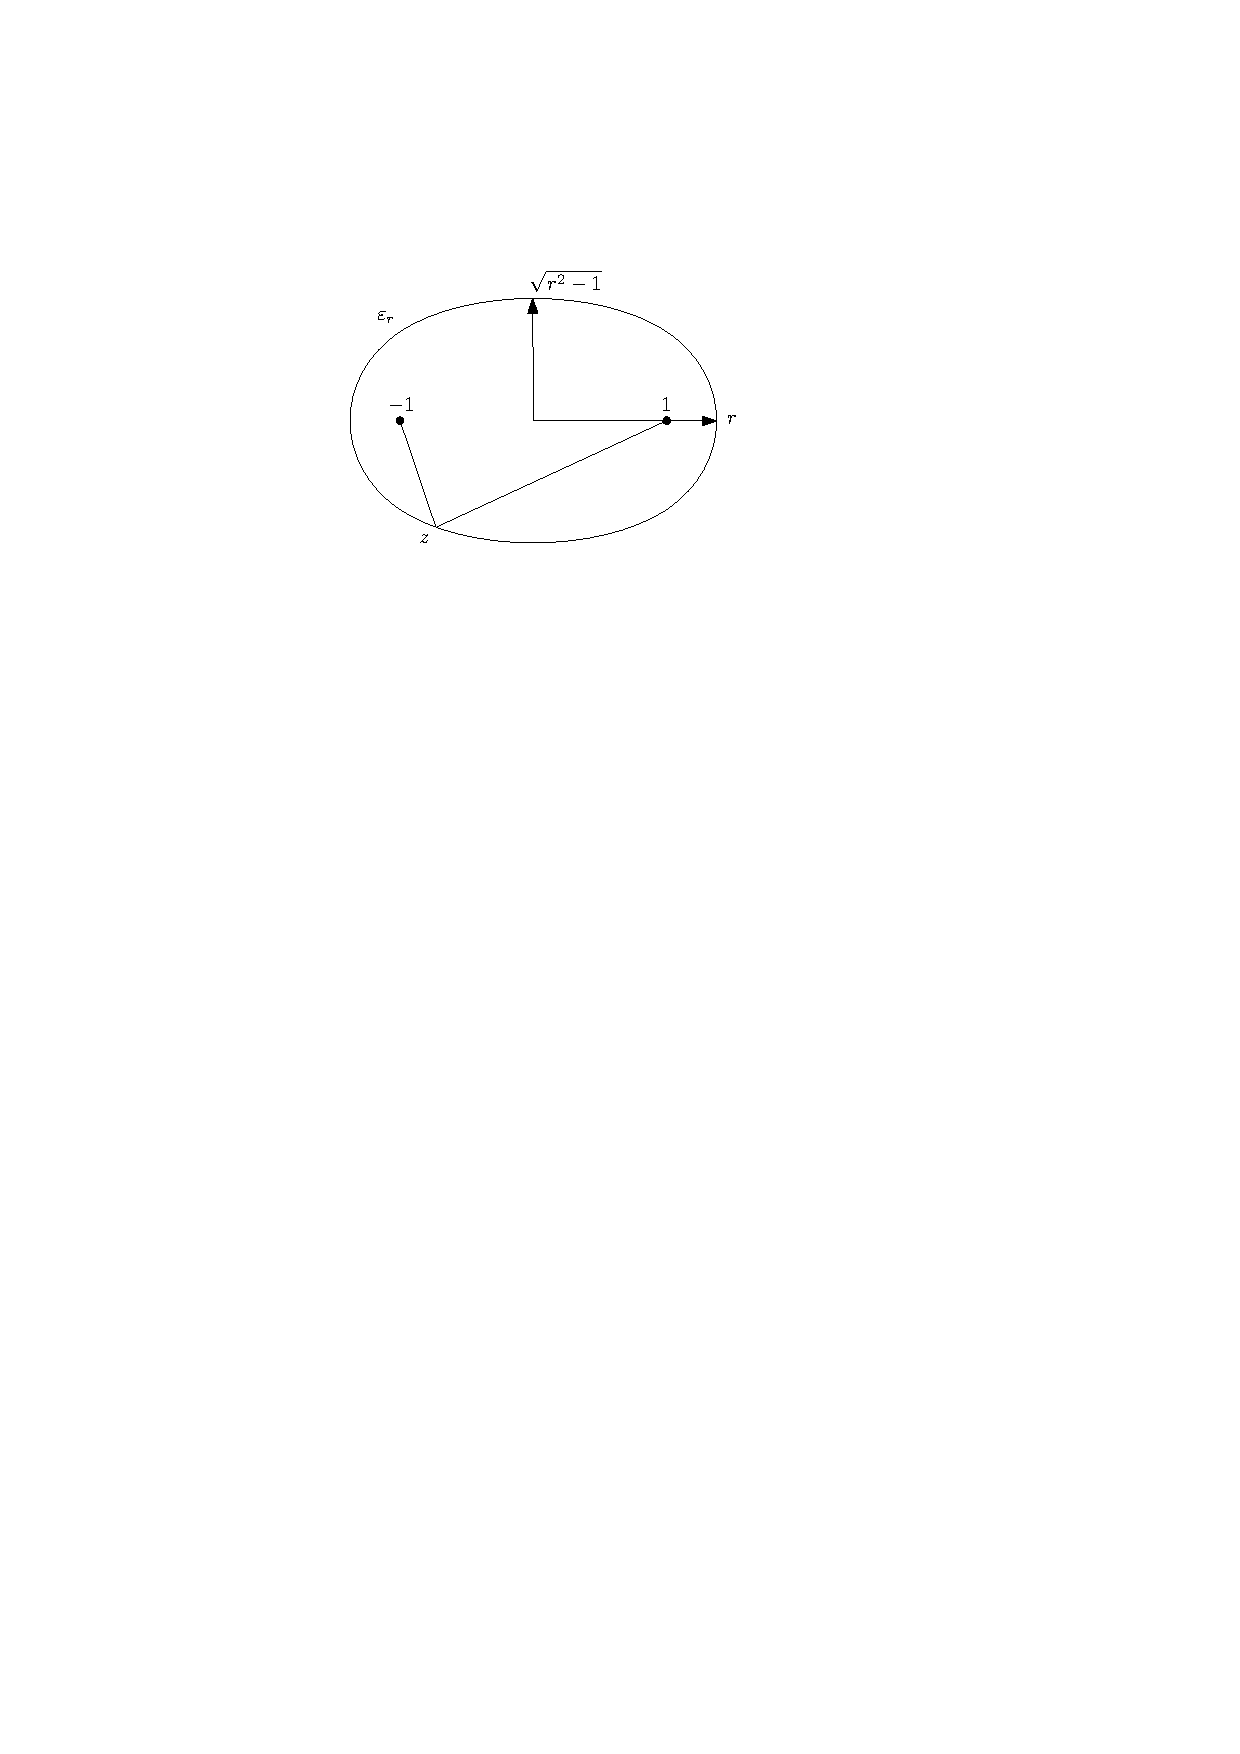
\includegraphics[width=5cm]{images/ellipse.pdf}
  \end{center} \caption{Ellipse parameters.}
  \label{fig:ellipse} \end{figure}

   \subsection{Implementation tricks}

   Here we simply give some further ideas used in our implementation to improve constants.

   \subsubsection{Improving branch points}

   As we saw in Section \ref{m-sec:numerical_integration}, the number of integration points
   closely depends on the configuration of branch points.

   In practice the tau constant of double-exponential integration is usually bigger than $0.5$
   for random points, but we can exhibit bad configurations with $τ\approx 0.1$. In this case
   however, we can perform a change of coordinate by a Moebius transform
   $x\mapsto \frac{ax+b}{cx+d}$ to redistribute the points more evenly.

   Improving $τ$ from $.1$ to say $.6$ immediately saves a factor $6$ on the running time.

  \subsubsection{Computing mth roots}
  \label{sec:computingroots}

  For numerical integration of the integrals in \eqref{m-eq:thm_periods_1}
  we need to evaluate $\ytab(u) = \prod_{x_k \ne a,b} (u-u(x_k))\mr$ at $u
  \in [-1,1]$. Instead of computing $(d-2)$ $m$-th roots for each
  integration point, we compute $q \in \frac12\Z$ such that $$\prod_{x_k \ne a,b}
  \left(u - u(x_k) \right)\mr = \zeta^q \cdot \left( \prod_{x_k \ne a,b}
  \left( u - u(x_k) \right) \right)\mr ,$$ which can be done by tracking
  the winding number of the product while staying away from the branch cut
  of the $m$-th root.

  For complex numbers $z_1,z_2 \in \C$ we can make a diagram of
  $\frac{\sqrt[m]{z_1}\sqrt[m]{z_2}}{\sqrt[m]{z_1z_2}} \in \{ 1, \zeta,
  \zeta^{-1} \}$, depending on the position of $z_1,z_2$ and their product
  $z_1z_2$ in the complex plane, resulting in the following Lemma.

  \begin{lemma}\label{lemma:wind_numb}
  Let $z_1,z_2 \in \C  \setminus  ]\infty,0[$. Then,
  $$\frac{\sqrt[m]{z_1}\sqrt[m]{z_2}}{\sqrt[m]{z_1z_2}} = \begin{cases}
                                                           \zeta, \quad \text{if} \quad \Im(z_1), \Im(z_2) > 0 \quad \text{and} \quad \Im(z_1z_2) < 0 , \\
                                                           \zeta^{-1}, \text{if} \quad \Im(z_1), \Im(z_2) < 0 \quad \text{and} \quad \Im(z_1z_2) > 0 , \\
                                                           1, \quad \text{otherwise}.
                                                         \end{cases}$$
   For $z \in ]\infty,0[$ we use $\sqrt[m]{z} = \zeta^{\frac{1}{2}} \cdot \sqrt[m]{-z}$.
  \end{lemma}
  \begin{proof}
   Follows from the choices for $\sqrt[m]{\cdot}$ and $\zeta$ that were made in \S \ref{m-subsec:roots_branches}.
  \end{proof}
   This Lemma can easily be turned into an algorithm that computes $q$.

   \subsubsection{Doing real multiplications}

   During integration, the main complexity comes from the multiplication by numerator
   $x_k=u_k-\frac{a+b}2$, which is usually done $g-m-1$ times for each of
   the $n$ integration points.

   More precisely, as we saw in the proof of Proposition \ref{prop:holom_diff}, for each power $j$
   we use the powers $0\leq i\leq d_i = \floor{\frac{dj-δ}m}$, with $\sum d_i = g$.

   However $x_k$ is a complex number while $u_k$ is real, so it is better to compute
   the integrals with $u_k$ only and make a simple shift on the integral values of the form
   \begin{equation}
       %\left(
       \int_{-1}^1 (u+c)^iF_j(u) \du
       %\right_{0\leq i\leq d_i}
       =
       %\left(
       \sum_{l=0}^i c^{i-l} \int_{-1}^{1} u^lF_j(u)\du
       %\right_{0\leq i\leq d_i}
   \end{equation}

   This saves a factor almost $2$ on the running time.

\biblio
\end{document}
